%%%%%%%%%%%%%%%%%%%%% RJT TeX Template %%%%%%%%%%%%%%%%%%%%%
\documentclass[oneside,11pt,a4paper]{article}

%%%% BHAM PREAMBLE - SET THIS FIRST! %%%%
\newcommand{\bhamstudentname}{Zhangda Xu}
\newcommand{\bhamthesistitle}{Curling with Deep Reinforcement Learning}
\newcommand{\bhamfronttitle}{Curling with \\ Deep Reinforcement Learning}
\newcommand{\bhamschool}{School of Computer Science}
\newcommand{\bhamcollege}{Engineering and Physical Sciences}
\newcommand{\bhamdegree}{Advanced Computer Science}
\newcommand{\bhamid}{2088192}
\newcommand{\bhamsupervisor}{Mohan Sridharan}
\newcommand{\bhamyear}{2020}
%%%%           %%%%


\usepackage[hyphens]{url}
\usepackage[breaklinks]{hyperref}
\usepackage{fancyhdr}
\usepackage[sort]{natbib}
\usepackage{comment}
\usepackage{dirtree}
\usepackage{longtable}
\usepackage{algorithm}
\usepackage{algorithmic}

\renewcommand{\algorithmiccomment}[1]{#1}

\pagestyle{fancy}
\renewcommand{\sectionmark}[1]{\markboth{#1}{}}


\lfoot{\bhamstudentname}
\cfoot{\thepage}
\rfoot{}
\fancyhfoffset[L]{0cm}
\newcommand{\HRule}{\rule{\linewidth}{0.5mm}}
\renewcommand{\headrulewidth}{0pt}
\newcommand{\tab}{\hspace*{1.25em}}
\newcommand{\minitab}{\hspace*{0.25em}}

\usepackage{perpage}
\MakePerPage{footnote}
\renewcommand*{\thefootnote}{\fnsymbol{footnote}}

\lhead{}\chead{}\rhead{\bfseries Curling with Deep Reinforcement Learning}
\setlength{\headheight}{28pt}
\setlength{\headsep}{6pt}
\pdfoutput=1
\usepackage[left=2.55cm,right=1.6cm,top=1.8cm,bottom=1.8cm]{geometry}
\usepackage{titling}
\setlength{\droptitle}{-2.75cm}
\usepackage{titlesec}
\titleformat*{\section}{\large	\bfseries}
\titleformat*{\subsection}{\normalsize \bfseries}
\titleformat*{\subsubsection}{\small \bfseries}

\titlespacing*{\section} {0pt}{3.5ex plus 1ex minus .2ex}{2ex plus .2ex}
\titlespacing*{\subsection} {0pt}{2.25ex plus 1ex minus .2ex}{0.75ex plus .2ex}
\titlespacing*{\subsubsection}{0pt}{2.ex plus 1ex minus .2ex}{0.5ex plus .2ex}

\setlength{\intextsep}{0pt}

\usepackage[pdftex]{graphicx}
\usepackage{enumitem}
\usepackage{pdfpages}
\usepackage{lastpage}
\usepackage{amsmath}
\usepackage{amsfonts}
\usepackage{amssymb}

\usepackage{epstopdf}

\usepackage{listings}
\lstset{
 basicstyle=\ttfamily,
  columns=fullflexible,
  keepspaces=true,
breaklines=true
}

\newcommand{\todo}[1]{\textcolor{red}{TODO: #1}\PackageWarning{TODO:}{TODO found: #1!}}

\DeclareGraphicsExtensions{.jpg}

%%%%%%%%%%%%%%%%%%%%%  END of TEMPLATE %%%%%%%%%%%%%%%%%%%%%


\title{MSc. Project\\\bhamthesistitle}
\author{\textsf{\bhamstudentname }}

\date{}
\begin{document}

\pagenumbering{arabic}
\begin{titlepage}
\begin{center}
\begin{minipage}{6in}
  \centering
  \raisebox{-0.5\height}{
\includegraphics[width=1.25in]{crest}}
  \hspace*{.2in}
  \raisebox{-0.5\height}{
\includegraphics[height=0.9375in]{uni}}
  \end{minipage}
  \\ [1.0cm]
\textsc{{\LARGE \bhamschool\\}College of \bhamcollege}\\[3.5cm]

\textsc{\Large MSc. Project}\\[0.5cm]

% Title
\HRule \\[0.4cm]
\begin{center}\Huge
\bhamfronttitle
\end{center}
\HRule \\[1.5cm]

\begin{center}
Submitted for the degree of MSc. \\ \textbf{{\large \bhamdegree}}\\
\vspace{1.5cm}
{\Large \textbf{\bhamstudentname}}\\
Student ID: \bhamid\\
\vspace{1.5cm}
{\Large Supervisor: \bhamsupervisor}
\end{center}
\vfill

% Bottom of the page
{\large September \bhamyear}

\end{center}
\end{titlepage}

% Table of Contents
\clearpage
\maketitle
\vspace{-5.5em}
\begingroup
\fontsize{9pt}{11pt}\selectfont
\tableofcontents
\endgroup
\clearpage
\phantomsection



\section{Abstract}

The problem that this project aims to solve is one of the task completion for intelligent agents in a tabletop environment. In the context of a practical setting, the agent learns to play curling on the surface with an improved control policy when observing the environment. Works in the project is intended to explore the application of various theoretical approaches in the field of reinforcement learning. The method proposed here takes in the rendered observation of environment directly as pixel input, and learn through deep neural networks end-to-end with returned policies. To simulate physics and conduct the experiments, we uses PyBullet \cite{pybullet} engine as an simulated environment with models of objects. Curling game play involves continuous control over the agent. The algorithm used for the task needs to update agent's deterministic policy for the given scenarios to improve convergence. During the training process, the agent is enabled to learn from past experiences of play to update current policies using a memory buffer. We propose an application with an \textit{actor-critic} architecture, integrating the deep deterministic policy gradient method with substantial improvements over existing issues. We show that our model can be successfully applied on the curling game play task like other classic reinforcement learning tasks. Comparing with existing state-of-the-art methods, the result indicates the improvement in stability and generalisation due to the proposed modification.
\vspace{0.5cm}

\section{Introduction}

The problem of agent control often involves the interaction with the environment. The goal here is to make good sequential decisions of actions given arbitrary situation of the environment. It is natural to consider both the agent and the environment it locates when control problem is to be solved. However, from the agent's perspective, the mechanics behind the world is often not known or incomplete, which makes it inapplicable for planning and prediction tasks. Instead, the agent needs a \textit{try-and-error} approach to learn from interactions with the environment, improving its own knowledge of the environment and how to choose actions next time. It is proved that agent is always able to improve the control through learning.
\newline
\newline
\noindent
The problem of learning is one of the most studied fields in machine learning. By definition, learning for an intelligence refers to the process of putting together a sequence of thoughts and actions, assisted by perception and observation of the environment. Artificial learning behaviour is similar to that of animal's. Generally, we have three paradigms to solve the learning problem: supervised learning, unsupervised learning and reinforcement learning. In supervised learning, the learner is trained with pre-labelled data to predict the result or labels given the raw input. We judge the performance of learner's predictions by comparing it with given results of known samples, where the feedback is often in the form of an optimisation term, or a similarity ratio. Unsupervised learning requires no prior knowledge of the labels of data, but only exploit the internal relationship between the data. On the whole, both approaches assume the data collected for prediction tasks to be identically and independently distributed. When is faced with the control task, both paradigms cannot fit properly for the purpose of sequential decision making.
\newline
\newline
\noindent
Reinforcement learning provides a better method to model the agent control task. A reinforcement learning world splits off the agent from its surrounding environment that out of the agent's control. The interactions between agent and environment are considered in a sequence of time steps. At every time step, the environment emits a scalar reward as the feedback, but no supervisor is needed. The reward signal is the goal of a reinforcement learning problem, which is analogous to positive or negative experiences of the agent. Thus the process of control is formulated as consecutive maximisation of the total reward. In addition, reinforcement learning enables the usage of correlated data obtained at different time, whose distribution is not invariant through learning.
\newline
\newline
\noindent
In this project, we propose to study the control of curling game play. Curling is a sports game where players in both teams slide stones on a sheet of icy surface toward a target area, which is segmented into four concentric circles. The smaller the circle is, the more the stones in it will score at the end of a game. The goal of the competition is to beat the other team in total scores on the ice. Each team takes turns to complete a round of throwing, with one player responsible for the throw and others responsible for sweeping on the ice to control the path of stone. There are various strategies for curling game play. Sometimes the key to victory lies not only in the precision of throwing, but rather to harass the positioning of opponent's stones. It is reasonable to pave the way for a better opportunity in the next round as well.
\newline
\newline
\noindent
The task of curling considered in the project is simplified to be a single round throw without assistant sweeping. By isolating decision making in consecutive rounds, we ignore the higher-level competitive game play consideration at this stage, focusing on the optimisation of throw control only. The problem of controlling the agent thus becomes: to search for the best initial velocity and angle of throw given the current positioning of friendly and opposite stones on the court, i.e. the best policy to play this round. Note that the actions to choose will be on a continuous space, if we look for a fine control on the agent.
\newline
\newline
\noindent
Recent advances in deep neural network makes it possible to learn the control policy directly from sensory inputs, such as high-dimensional visual data. Deep multi-layer perceptrons are capable of extracting high-level representations of the original data, which make hand-picked features obsolete. In order to learn end-to-end, we need to make use of the agent's observations of the environment to discover the optimal policy. However, reinforcement learning takes the try-and-error approach, which may incur unrecoverable repercussions in physical experiments. On the other hand, the captured vision or speech is often too noisy to use for learning task. We avoid these obstacles by using a simulated environment in PyBullet, where all the physics are handled with by the engine and visuals are rendered as the final output. Most parts of the software will be implemented in this ecosystem.
\newline
\newline
\noindent
This project is intended to solve the problem of curling game play using deep reinforcement learning. This report first establishes the theoretical ground of using such technique, and concludes the previous related work for comprehensive insights. Then, we formulate the state-of-the-art solution for similar problems and show that practical improvements are required for this specific task. The implementation of the whole architecture is discussed in detail. We later present the experiments of the proposed algorithms and compare it with existing variants. We finally evaluate the results in depth and validate the proposed methods. The software developed so far in this project is able to visualise the process of training and simulations. The performance of the algorithm is proved to be stable and outperform the average human player.
\vspace{2cm}
\begin{center}
    \includegraphics[scale=.15]{curling.png}\\
    Figure 1: Curling sheet \cite{curlingmap}
\end{center}

\newpage
\section{Preliminaries}
In this section, we introduce the preliminaries needed to formulate both the problem and solutions in reinforcement learning.

\subsection{Reinforcement Learning}
In a reinforcement learning paradigm, we consider the control task of the cue stone interacting with the environment of a curling court. The agent can be thought as a self-controllable intelligent stone or an external robotic arm that exerts an initial push on it. In either case, at each time step $t$, the agent selects an action from the space of all legit actions $a_t \in\mathcal A$, given the current state $s_t \in \mathcal S$. Since the internal state of the environment is not known to the agent, we treat the observation of the simulated environment $\mathcal O$, which is rendered from a stationary point of view, as a full representation of the state. As a response to the agent, the emulator then emits a reward $R_t$ and the new state $s_{t+1}$ after receiving the action-state pair. A basic representation of reinforcement learning can be given as a tuple:
$$
\left\langle \mathcal {S,A, R} \right\rangle
$$
The reward $r_t$ is a feedback signal which indicates how well the agent is doing at time step $t$. Although it is arbitrary to design the reward signals, the reward hypothesis states that all goals of the agent should be described by the maximisation of expected cumulative reward. The instant reward in the current state $R_t$ for an action $a_t$ alone is not a complete feedback of how good the action is, because it ignores its potential effects on the environment and the following states. We instead define the return $G_t$ of an episodic task as the total discounted reward starting from time step $t$:
$$
G_t = R_{t+1} + \gamma R_{t+2}, +\gamma^2 R_{t+3}+... = \sum_{k=0}^\infty\gamma^kR_{t+k+1}
$$
Here $\gamma$ is a discount parameter applied to every consequent reward in the future, where each component represents the present value of future rewards. We use the discounted version of the total reward for several reasons. First, it correctly models the uncertainty about the future in the process. It also incorporates the common preference of immediate reward over delayed ones. Lastly, it can avoid infinite returns for cyclic process. \cite{ds}
\newline
\newline
\noindent
\subsection{Markov Decision Process}
We next formulate the environment of reinforcement learning with Markov decision process. A state is considered Markov if and only if the current state captures all relevant information from the history. It means that given the current state, to predict the future states, all the previous history can be thrown away. In the form of a conditional probability, the next state is independent of past history:
$$
\mathbb P[S_{t+1}|S_t]=\mathbb P[S_{t+1}|S_1,...,S_t]
$$
A Markov decision process is where all the states are Markov. Most reinforcement learning problems can be simplified as MDPs so that there is no need for deduction of what happened in the past. In a tabular representation, the probability of each possible successor state is described by the state transition matrix:
$$
\mathcal P_{ss'}^a=\mathbb P[S_{t+1}=s'|S_t=s, A_t=a]
$$
The goal in MDP is to find the best behaviours for the agent in the face of different states. We define the policy $\pi$ as a mapping of actions given states:
$$
\pi(a|s) = \mathbb P[A_t=a|S_t=s]
$$
Since the state is a sufficient statistic for the environment, the policy is a stationary distribution of behaviours given the state: $A_t \sim \pi(\cdot|S_t)$. We can use the policy to rewrite the reward function following a fixed policy in a form of expectation:
$$
\mathcal R_s^\pi = \sum_{a\in \mathcal A}\pi(a|s)\mathcal R_s^a
$$

\subsection{Value Functions}
Recall that the purpose of an agent in reinforcement learning is to maximise the expected value of the total reward. We can formulate the state-value function of a state $s$ under a policy $\pi$ as the expected return starting from the current state, following policy $\pi$:
$$
V_\pi(s) = \mathbb E_\pi[G_t|S_t=t]
$$
The action-value further incorporates the value of actions into the value of current state, which is often preferred in reinforcement learning problems because it is solely dependent on the environment. Similarly, it describes the value of taking action $a$ given a state $s$, following a policy $\pi$ in next steps:
$$
Q_\pi(s,a) = \mathbb E_\pi[G_t|S_t = t, A_t = a]
$$
Due to the recursive property of the return, we can decompose the return at time-step $t$ into an immediate reward and the expected value of successor states. This one-step look-ahead can be used as the update rule of action-values, which enables the recursive evaluation of current policy. This is known as the Bellman equation:
$$
Q_\pi(s_t,a_t) = \mathbb E_\pi[R_{t+1} + \gamma\mathbb E_\pi [Q_\pi(s_{t+1}, a_{t+1})]]
$$
Here the expectation of the action-value given the current state-action pair is the backup of the complete transition, where every successor state is used in a sweep recursively until the end of episode. Although the Bellman update makes use of dynamic programming to reduce space complexity, it still causes huge cost of unnecessary memory. This requires a full backup of the entire process, including the knowledge of complete transitions and rewards. In practice, it is hardly known to the agent. Instead, the agent needs to learn from episodes of its experience.
\vspace{0.25cm}
\noindent
Temporal-difference learning is a policy evaluation method that can learn from incomplete sequences without the model of Markov decision process. \cite{td} It explores the Markov property of states using bootstrapping and sampling simultaneously. Like the Monte Carlo method, TD learning uses sampled episodes instead of an exhaustive search to approximate the expectation term in the equation, in which a full process is explored until the terminal state. TD learning is also bootstrapping, which enables it to learn from incomplete episodes even without the final outcome. The main idea is to update the functions towards another belief of the state. Consider the simplest variant TD(0), the algorithm updates the value function $V(s_t)$ online towards an estimated return at the next time-step:
$$
V(s_t)\leftarrow V(s_t)+\alpha(R_{t+1}+\gamma V(s_{t+1})-V(s_t))
$$
Here $R_{t+1}+\gamma V(S_{t+1})$ is the TD target, $\alpha$ is the step parameter, which ensures continuous update towards the TD target. It can be proved that TD(0) converges to solution of maximum likelihood estimate of Markov model that best fit the data. Temporal-difference learning introduces bias to the estimate but lowers the total variance, because the TD target only depends on one state transition and reward, which can be a result of poor state representation. It is also a much cheaper online update scheme in large scale problems. TD learning accelerates the process of learning by exploiting the state property of a Markov decision process.
\newline
\newline
\noindent
\subsection{Q-learning}
It is essential for the agent to improve the policy starting from an initial action. It is necessary for the agent first to evaluate the policy, then updates it iteratively towards the best policy. For any Markov decision process, there always exist one or multiple policy $\pi^*$ that is no worse than any other policies. In general policy iteration processes, the optimal policies are guaranteed to achieve the optimal action-value. This gives us the description of optimal action-value function in Bellman equation:
$$
Q^*(s,a) = \mathbb E[r(s,a) + \gamma\max_{a'} Q^*(s',a')]
$$
If we can solve $Q^*(s,a)$, we can solve the optimal policy by directly assigning the optimal action $a^*(s)$ as:
$$
a^*(s) = \arg\max_aQ^*(s,a)
$$
Off-policy learning method promises usage of data collected at any time step during training for update. One of the most famous algorithm in this family is Q-learning or Sarsa-max. Basically, the aim is to learn an approximated optimal action-value function $Q_\theta(s,a)\approx Q^*(s,a)$, which is able to generalise to unseen states. It uses an objective function based on mean squared Bellman equation error. In a TD learning update, the Q-learning target is simply to be the next action that maximises the action-value in next states: $r(s,a) + \gamma\max_{a'} Q^*(s',a')$. The TD control of Q-learning is thus a fixed step update to the target:
$$
Q(s,a) = Q(s,a) +\alpha[r(s,a)+\gamma\max_a Q(s',a) - Q(s,a)]
$$
Q-learning directly learns the optimal approximated action-value function independent of the policy it followed. This property enables faster convergence of the process. Here the maximisation over an estimate is considered equivalent to an estimate of the maximum value. We show in later sections that this introduces a positive bias in many cases and causes an systematic over-estimation of the action value.
\newline
\newline
\noindent
\subsection{Policy Gradient}
Value-based policy iteration improves the policy by acting with respect to the value function. Alternatively, we can directly learn the parameterised policy. In many occasions, value-based policy iteration approaches are unstable to converge to the optimal policy due to the sparse value distribution. The values are not reliable to learn the target policy when stochastic decision making is needed. Moreover, value-based policy improvement cannot effectively model actions in high-dimensional or continuous spaces. Policy-based reinforcement learning promises an optimisation problem over the whole action space. On the other hand, the evaluation of policy is often inefficient and introduces high variance in the process.

\noindent
The key aspect of policy gradient is to essentially increase the probabilities of choosing actions leading to higher return, while lowering down the probabilities of choosing inferior actions. Policy gradient algorithms can be formed as an optimisation problem searching for a local maximum of a policy objective function. \cite{pg} The quality of policy, or the scale of objective, is often related to the rewards in one episode. The gradient describes the direction and the magnitude of most effective ascent of one step update. Policy is updated online using gradient ascent with respect to the parameters. For an approximated policy $\pi_\theta$, with a fixed step size $\alpha$, the updated value of parameters $\Delta \theta$ is given as:
$$
\Delta\theta=\alpha\nabla_\theta J(\theta)
$$
Here $\nabla_\theta J(\theta)$ is the policy gradient, which can be calculated analytically. A common practice is to rewrite the original gradient as an expectation of the log probability of the gradient:
$$
\nabla_\theta J(\theta) = \pi_\theta(s,a)\cdot\nabla_\theta \log\pi_\theta(s,a)
$$
Policy gradient theorem states that for a differentiable policy $\pi_\theta$ approximated by parameters $\theta$ and any policy objective, the policy gradient is given as:
$$
\nabla_\theta J(\theta) = \mathbb E_{\pi_\theta}[\nabla_\theta\log\pi_\theta(s,a)Q^{\pi_\theta}(s,a)]
$$
Here $Q^{\pi_\theta}(s,a)$ is a long-term value for the policy. Policy gradient in the form of an expectation makes it convenient to use stochastic gradient ascent optimisation. It improves the convergence of the policy optimisation process. Naive policy gradient is an on-policy algorithm, which updates according to current policy. The algorithm promises a stochastic policy for the agent at the start. However, the policy often becomes less random eventually all along the training process. It is encouraged by updating the policy with to existing rewards, which raises the problem of trapping in the local optima.

\newpage
\section{Method}


We next formulate the curling play problem and iterate over the learning approach with further exploration into state-of-the-art algorithms towards the objective.

\subsection{Problem Formulation}
The problem of curling game play generally deals with the task of sliding a cue stone towards a target area in a controlled manner. The stone is initially stationed at the centre of a house. The goal of the task is to achieve the highest score in another house on the sheet of ice. Curling is a game played by two teams of players, which involves competition and cooperation consistently. We here simplify the case where only one throw is considered. The agent is aimed to learn the control policy for sliding the cue stone such that after the release, the trajectory of stone leads to a better score given the current scenario on the ice. The scoring rules stipulate that the score of the winning team in each round is the number of stones closer to the centre of house than the opponent's closest stone. Since the score on the court is determined before the throw, the goal of the agent is equivalent to achieving the most score after one throw. Each team takes turn to play 8 stones in a round. Thus there are no more than 15 stones on the sheet for the agent. When the team with the closest stone wins, the other team scores 0. However, we can still differentiate the result with the advantage and loss in scores over the opposite team. The goal is thus to maximise the difference of scores in a round after the throw. Suppose the distance from every friendly stone $m_i$ and opposite stone $n_i$ to the centre of house $c$ is denoted as *dist(~,c)*, the reward $R_t\in[-8,8]$ is determined by the number of stones that satisfy:
$$
dist(m_i, c) \in (\min_i dist(n_i, c), \min_j dist(m_j, c)]
$$
The agent is trained to finish a task where different situations exist. For instance, when the agent is the lead, i.e. the first to play in a round, the goal of this task is essentially to learn the control of how to slide the stone to the house centre. When no opposite stone exists, the ideal strategy is to maximise the total score of all friendly stones. The priority changes if at least one opposite stone is closer to the centre, because the only way to win the round is to kick off the closest opposite first. Other strategies emerge with more stones on the sheet, where either approach gains advantage over the opposite. The learnt policy should deal with a generalised set of situations discussed.
\newline
\newline
\noindent
The agent is faced with a fully observed environment where the observation $O_t$ is a sufficient statistic for the state $S_t$. We consider the state of environment in a planar setting, while the physics is simulated completely. The observation space is totally defined by the rendered view of the state after a throw, which is a RGB matrix: $s_t \in \mathbb R^2$. We define the actions as choosing the initial force on the direction of both orthogonal axes: $a_t\in \mathbb R^2$. The Newton's law describes the correlation between acceleration and an external force as $F=ma$. In this special case, we assume that the duration of acceleration exerted on the stone is a constant $T$ throughout all the games. This process is constrained by the hog line, where the stone must be released.
\newline
\newline
\noindent
Learning of such policy requires a deep representation of the visual input, and an effective convergence in the continuous action space. Given a processed input $\phi(s_t)$, we look for the optimal parameterised policy $\mu_\theta(\phi(s_t))$ that selects an action over a continuous space, which maximises the total return $G_t$.
\newline
\newline
\noindent
\subsection{Related Work}
The temporal-difference learning method with function approximation is one of the most important development in reinforcement learning. With a linear function approximator, the TD learning is proved to converge over the horizon of a Markov process. Policy gradient method proposed by Sutton sets down the ground for families of modern RL algorithms, especially in continuous action space. Actor-critic methods follow a generalised policy iteration. The architecture evolves with different definition of actor and critic.
\newline
\newline
\noindent
The use of convolutional neural network to extract information from images is a great breakthrough in the domain of deep learning. A ConvNet structure is commonly used in computer vision and voice recognition problems, consisted of a convolutional filter, a ReLU activation and a fully-connected layer. The first deep Q-learning method is applied in an Atari game environment. Such artefact has low resolution visual output, which is easy to learn an approximator using neural network.
\newline
\newline
\noindent
A recent work applies the deep Q-learning method to improve the striking accuracy in air hockey. \cite{puck} The control task of strike follows a customised reward based on properties of the hit puck. It discretises the action space using a sampled 2-dimensional grid to follow the DQN scheme.\cite{atari}
\newline
\newline
\noindent
The Q-learning algorithm uses a greedy maximisation step to select the action. It is widely known to over-estimate the action values in many situations. Many previous work address the systematic problem found in their environments. Further investigation proves that it exists in deep Q-learning and actor-critic algorithms. \cite{ac}
\newline
\newline
\noindent
Recent researches incorporate the evolution strategies \cite{es}into the RL problem. They enable a parallelised learning process over different targets. The development of GPU computation makes it a suitable optimisation scheme for large-scale problems.
\newline
\newline
\noindent
\subsection{Actor-Critic}
In section 2.4 and 2.5, two families of model-free reinforcement learning algorithms are introduced. They are used to deal with situations where the agent has no access to or the internal model of the environment, which is often the case in practice. Instead, the agent itself learns to improve the action selection with respect to the feedback received. Q-learning control methods learn to act according to action-value functions, which are often performed off-policy. Policy gradient methods directly optimise the policy it acts on. Optimisation of policy gradient requires an on-policy update, which only makes use of data collected under the most recent policy.
\newline
\newline
\noindent
We must consider the trade-offs between Q-learning and policy optimisation paradigms. Agents following a Q-learning approach indirectly optimise the performance based on the comparisons of interpreted values. It causes failures or instability in many models, but learning off-policy is essential in many problems because it allows learning of different target policies, even those from other agents' experiences. Policy optimisation methods make use of the gradient of policy to directly improve the final output. This optimisation approach is widely used in the paradigm of supervised machine learning  and proved to be reliable in most cases. It is opportune to inherit both the sample efficiency from Q-learning and stability from policy optimisation methods.
\newline
\newline
\noindent
Actor-critic algorithm is an framework that integrates value-based evaluation to policy gradient methods. At the first step, we represent the policy $\pi(a|s,\theta)$ as a differentiable parameterised distribution of action-state pairs. To address the variance in policy gradient optimisation, we can also estimate the action-value function under parameterised policy $\pi_\theta$ using a critic: $Q_w(s,a)\approx Q^{\pi_\theta}(s,a)$. A critic is the supervisor that review the performance of a modelled task. It is responsible of the job to update the parameters of action-value function $\mathbf w$ with respect to the TD target $\delta$ following the value-based approach. We then define an actor that updates the parameters of our policy in the direction suggested by the critic. This follows one step of gradient ascent as in policy-based methods. Two general update rules of an actor-critic architecture over two parameters $\mathbf w, \mathbf \theta$ are given below:
$$
\delta = r + \gamma Q(s',a') - Q(s,a)\\ \theta \leftarrow \theta +\alpha\nabla_\theta\log\pi_\theta(s,a)\delta \\ w\leftarrow w+\beta\delta Q_w(s,a)
$$
Here $\alpha, \beta$ are the step size for two updates, respectively. Actor-critic follows an approximated policy gradient in the form of an expectation, which allows stochastic gradient methods and efficient sampling. The difference in policy parameters is proportional to the error term suggested by the critic. In many cases, the action-value function can be replaced by a baseline function. Actor-critic provides a better approach for the convergence of optimisation.
\newline
\newline
\noindent
\subsection{Deep Reinforcement Learning}
Last sections conclude the modelling of a tabular representation of reinforcement learning problems. The whole process is stored as pairs of state and action, where the value of each state is calculated individually. Recent development in sensory data processing requires an efficient architecture for large-scale problem solving. It is common to approximate the functions with parameters, such as linear functions and neural networks, to generalise the problem from known states to unseen states.
\newline
\newline
\noindent
Recent development in deep neural network introduces new approaches to reinforcement learning. In this project, we use MLP as a non-linear function approximator of state-value function. A feed-forward neural network was first proved to be an universal approximator by Cybenko in 1989. It means that a multi-layer perceptron with at least one hidden layer is able to represent any mapping from the input data to an output. This is achieved by introducing non-linear transformation with an activation function. The value of a neuron is the weighted sum of the values in previous layer with a local bias. The output is then activated and used for further feed-forward update. A multi-layer perceptron (MLP) with activation function $\phi$ can be represented by weight matrices $W_h, W_o$ and arrays of bias $b_h, b_o$ of the hidden layer and output layer, respectively:
$$
\mathbf {H = \phi(XW_h + b_h) \\
    O = HW_o+b_o}
$$
The goal of this project is to solve the reinforcement learning problem end-to-end. We connect the processing of input data and the reinforcement learning algorithm together, which returns the optimised policy after episodes of training. Inspired by computer vision, the RGB rendered image is filtered through a convolutional network as the pixel input. Convolutional filters slide over all spatial locations of an visual input and returns multiple activation maps. It is able to extract the local correlation of the image and keep a representation of details. The ConvNet architecture consists of a 2-dimensional convolutional layer, a rectified linear unit (ReLU) activation and a fully-connected layer. The ReLU activation removes negative values in pixels by replacing it with $max(0, w_hx_i+b_h)$, which solves the problem of vanishing gradient. The input is then fed into the policy network for optimisation. Learning end-to-end requires no hand-picked features or iteration of inference structure. It drastically accelerates the development and inference of a reinforcement learning model.
\newline
\newline
\noindent
Deep Q-learning is one of the most famous application of such architecture in an Atari game environment. \cite{atari} It reads the input directly from frames of screen and pre-processes the state representation for optimisation. A deep Q-network is used to represent the action-value function $Q_\theta$. DQN proposes a novel memory replay mechanic to improve the data efficiency. In every episode, a state transition $s\rightarrow s'$ is stored into a memory buffer $\mathcal D$ once finished in simulation, represented by a quadruple $[s_t,a_t,r_t,s_{t+1}]$. At each iteration, we apply the Q-learning update using samples of experience stored in the memory. At every time-step, the action is selected with respect to the Bellman optimality equation. Exploration in deep Q-learning is maintained by an epsilon-greedy policy, where with a small probability $\epsilon$, a random action is chosen over the optimal one. In non-terminal states, the objective is calculated as the Bellman error: $r+\gamma\max_{a'}Q_\theta(s',a')-Q_\theta(s,a)$. The variance introduced by the up-to-date parameters at each step may impair the stability of the architecture. Instead, DQN implements a target network with delayed but fixed parameters $\theta_{targ}$, which the target is then updated to. For every $\tau$ steps, parameters on the Q-network are copied onto the target network periodically. The final action-value of each discrete action is yielded separately after a single forward pass.
\newline
\newline
\noindent
\subsection{Deep Deterministic Policy Gradient}
Deep Q-learning proposes an efficient architecture for the learning of value functions using large-scale non-linear function approximators. The class of DQN algorithms solve the action-value separately in discrete action space. However, the curling play task we aim to solve in this project is formulated on continuous action spaces. Fitting the problem into DQN requires discretisation over the defined action space. It causes problematic constraints on the solution, such as the curse of dimensionality. The Q-learning approach of assigning the optimal action also need to iterate over the entire action space for the maximisation of action-value, which is not applicable on continuous space.
\newline
\newline
\noindent
We consider deep deterministic policy gradient algorithm to solve the problem. \cite{ddpg}DDPG is an algorithm that follows the DQN approach but applies an actor-critic architecture to a continuous action space. It updates the Q-network and a policy in an off-policy way. At every time step, the action is selected based on a deterministic parameterised policy $\mu_\theta(s)$. Following a deterministic policy can easily lead to a local optimum with insufficient exploration of the space. We add a random Gaussian noise $\epsilon \in \mathcal N(0)$ sampled at every iteration to the policy. It is a simple modification enabled by the continuous action space, which provides intrinsic stochasticity on all dimensions. The scale of this noise term remains fixed throughout the learning process.
\newline
\newline
\noindent
DDPG inherits experience replay method and a target network from deep Q-learning. The target network further smooths the parameter update by using Polyak averaging. The target parameters are softly updated towards the current setting. The value of hyper parameter $\rho$ is often chosen to be close to 1:
$$
\phi_{targ} \leftarrow \rho\phi_{targ} + (1-\rho)\phi
$$
The Q-learning update is to minimise the mean squared Bellman error loss with a stochastic gradient descent approach. The quadruple of a transition with a termination indicator $d$ is stored in the memory buffer, which cancels the later return if in a terminal state. In every update, it samples a random mini-batch of transitions for the optimisation of objective function parameterised by a target policy network $\phi_{targ}$:
$$
L(\phi, \mathcal D) = \mathbb E_{(s,a,r,s',d)\sim \mathcal D}[Q_\phi(s,a) - (r+\gamma (1-d)Q_{\phi_{targ}}(s', \mu_{\theta_{targ}}(s')))]
$$
Here the $\mu_{\theta_{targ}}$ is the target policy that learnt from stable optimisation. Learning process of the policy is based on the maximum action-value $Q_\phi(s,a)$. We assume that the Q-function is differentiable in the continuous space with respect to selected actions. The gradient ascent update is then performed over the policy parameter $\theta$ such that it solves the maximum action-value function:
$$
max_\theta \  \mathbb E_{s\sim \mathcal D}[Q_\phi(s, \mu_\theta(s))]
$$
\newline
\newline
\noindent
\subsection{Twin Delayed DDPG}
We explore deeper to improve the generalised performance and stability of DDPG with further detailed modification using Twin Delayed DDPG (TD3). \cite{td3}
\newline
\newline
\noindent
In DDPG algorithm, the learnt target policy follows an optimisation over current deterministic policy, which is approximated by a network. The target carries more weight than other parameters because it also determines the evaluation of action-value term in loss optimisation. As explained in section 2.4, the maximisation over the action-value in Q-learning is over-estimated. In continuous action space, the over-estimation further introduces a positive bias in the update.
\newline
\newline
\noindent
We need first to consider the action used to calculate the Q-learning target. In this problem, the action space is consisted of a pair of orthogonal forces. Before fine-tune the control of the stone towards the target area, the agent first needs to figure out the valid combination of exerted forces to avoid the side walls, which is a terminal state of no reward by rules. It is beneficial to first constrain the actions on a clipped interval, so that the stone first has to figure out the valid direction to the house out of all possible directions. The policy used for selection is also regularised with a clipped noise as in DDPG. Thus the target action is selected as:
$$
a'(s') = clip(\mu_{\theta_{targ}}(s') + clip(\epsilon,-c,c), a_l,a_h)
$$
In plain words, this modification avoids too deep pursuit of high-value actions that are not promising to the final task. The smoothing technique ensures that no sharp deviation exists among similar actions.
\newline
\newline
\noindent
We next address the problem of systematic over-estimation bias. In the TD3 paper, the authors prove that this bias exists in state-of-the-art actor-critic methods as well. Double Q-learning is an effective approach to avert it is to disentangle the evaluation of critic and selection of actor. Two groups of actors and critics are trained separately for the maximisation greedy step in Q-learning. The target is then clipped to be the smaller value from parameters $\theta_1,\theta_2$:
$$
y(r,s',d) = r+\gamma(1-d) \min_{i=1,2}Q_{\phi_{i,targ}(s',a'(s'))}
$$
Both actors are optimised with respect to the clipped target:
$$
L(\phi_1,\mathcal D) = \mathbb E_{(s,a,r,s',d)\sim \mathcal D}[(Q_{\phi_1}(s,a) - y(r,s',d))^2] $$
$$L(\phi_2,\mathcal D) = \mathbb E_{(s,a,r,s',d)\sim \mathcal D}[(Q_{\phi_2}(s,a) - y(r,s',d))^2]
$$
TD3 also proposes a less frequent update procedure for the policy than the action-value function. It shows that a delayed update can reduce the error raised by function approximation for the target networks, which is backed by empirical results in other papers. We modify the usage of the memory buffer $\mathcal D$ in TD3 by adding a lower bound of the number of samples for valid update. It means that at the starting steps, the agent is following a uniformly random policy over valid action space. The experience replay mechanic then takes over for later exploration. The pseudo-code of TD3 algorithm used in the experiment is listed below.
\newline
\newline
\noindent

\begin{algorithm}[H]
    \floatname{algorithm}{Algorithm I}
    \renewcommand{\thealgorithm}{}
    \caption{Twin Delayed Deep Deterministic Policy Gradient}
    \begin{algorithmic}[1]
        \STATE Initialise policy parameters $\theta$, Q-function parameters $\phi_1, \phi_2$, replay buffer $\mathcal D$.
        \STATE Record target parameters equal to current parameters $\theta_{targ} \leftarrow \theta, \phi_{targ,1} \leftarrow \phi_1, \phi_{targ,2} \leftarrow \phi_2$
        \STATE \textbf{Repeat}
        \STATE \hspace{0.5cm} Observe state $s$ and execute action $a=clip(\mu_\theta(s)+\epsilon, a_{Low}, a_{High})$, where noise $\epsilon \sim \mathcal N$.
        \STATE \hspace{0.5cm} Observe next state $s'$, reward $r$, terminal indicator $d$.
        \STATE \hspace{0.5cm} Store $(s,a,r,s',d)$ into the replay buffer $\mathcal D$.
        \STATE \hspace{0.5cm} If $s'$ is terminal, \textit{reset} environment $\mathcal E$.
        \STATE \hspace{0.5cm} \textbf{for} $t=1$ to $T$ \textbf{do}
        \STATE \hspace{1cm} Sample a random mini-batch of transitions $B = \{(s,a,r,s',d)\}_N$ from $\mathcal D$.
        \STATE \hspace{1cm} Compute target actions
        \begin{center}
            $a'(s') = clip(\mu_{\theta_{targ}}(s')+clip(\epsilon, -c, c),a_{Low}, a_{High}), \ \epsilon \sim \mathcal N (0,\sigma)$
        \end{center}
        \STATE \hspace{1cm} Compute the target
        \begin{center}
            $y = r+\gamma(1-d)\min_{i=1,2}Q_{\phi_{targ,i}}(s',a'(s'))$
        \end{center}
        \STATE \hspace{1cm} Update Q-functions by gradient descent for $i=1,2$
        \begin{center}
            $\nabla_{\phi_i} N^{-1}\sum\limits_{(s,a,r,s',d)\in\mathcal B}(Q_{\phi_i}(s,a) -y)^2$
        \end{center}
        \STATE \hspace{1cm} \textbf{If} $t \mod delay$ \textbf{then}
        \STATE \hspace{1.5cm} Update policy $\phi$ using deterministic policy gradient
        \begin{center}
            $\nabla_\theta N^{-1}\sum\limits_{s\in\mathcal b}Q_{\phi_1}(s,\mu_\theta(s))$
        \end{center}
        \STATE \hspace{1.5cm} Update target networks with Polyak $\rho$ for $i=1,2$
        \begin{center}
            $\phi_{targ,i}\leftarrow \rho\phi_{targ,i} + (1-\rho)\phi_i$
        \end{center}
        \begin{center}
            $\theta_{targ}\leftarrow \rho\theta_{targ} + (1-\rho)\theta$
        \end{center}
        \STATE \hspace{1cm} \textbf{end if}
        \STATE \hspace{0.5cm} \textbf{end for}
        \STATE \textbf{until} convergence

    \end{algorithmic}
\end{algorithm}
\vspace{0.5cm}

\section{Implementation}
This section introduces the overall architecture of implemented software and considerations in the development. The problem and algorithms used are well discussed in the last section, whose parameters will be discussed below.

\subsection{PyBullet Simulation}
We first present the construction of a reinforcement learning environment in PyBullet. Bullet is a physics simulation engine which is widely used for games, robotics and reinforcement learning. Newest version of the engine provides a simplified API in Python. The engine plays a key role in simulation and rendering in this project. No graphical user interface is supported in the control of software developed in this project.
\newline
\newline
\noindent
We consider the environment to be consisted of three main objects: the self-controllable puck, the ice sheet and other stones in the same form of the puck. The models are created in unified robotic description format, i.e. *.urdf* files. Basically, it describes all the necessary properties of a robot for collision and physics simulation. The sheet with icy surface is a resized anatomy to the real curling court, with three vertical walls blocking objects out of the designated area. The aspect ratio of the slide is 1:10. Two houses are located at both ends of the sheet, which are composed of 4 concentric circles with radii of 0.15m, 0.61m, 1.22m and 1.83m. Other components of the sheet is simplified for more efficient experiments. The friction on the sheet is the most important invariant physical property that could affect the curling play. Considering the simultaneous rotation and sliding of the stone, we set both the lateral and rotational friction coefficient of the sheet according to empirical statistics. Notice the centre of home base is set as the origin in coordinate system.
\newline
\newline
\noindent
The stones used by both teams are in the same form except colours. Geometrically, the stone is a short cylinder with rounded edges. The flat running surface at the bottom is about 3/4 of the outer diameter. We ignore the handle on real stones to build it in a regular shape. To improve the effectiveness of visual input, the friendly and opposite stones are painted with read and blue materials which can be easily distinguished in the white background of the ice sheet. The weight of each stone is set to be about 18 kg.
\newline
\newline
\noindent
The interactions between stones and environment are also confined within the simulator. The cue stone is programmed to be exerted with an initial push and a slight spin in each round. Due to the limitation of exact rotation simulation, we treat the spin as a random noise that out of the control of an agent. Thus the action space only considers initial velocity on the direction of orthogonal axes as a controllable task. The state of environment is rendered visually by the internal Bullet engine. We use a bird view camera to observe the entire scoring are on the curling court. The rendered image is then pre-processed as the 2-dimensional visual input of the model.
\newline
\newline
\noindent
Other standing stones are randomly positioned on the path to the house behind the hog line, i.e. the legitimate scoring zone. The number of stones on the sheet vary from 0 to 10, indicating different states that a player might face in the game. A clear curling sheet means the goal is simply to figure out how to throw the stone to the centre of house. A more complex scenario with stones from both sides incurs strategies of a single throw. The stone can be used to *promote* another friendly stone or knock out the enemies. Notice that common strategies in real-world curling include playing guardian stones that can protect scoring stones in the house from opposites. Such adversarial move is a result of continuous competitive game, which is ignored in the single round curling play.
\newline
\newline
\noindent
\subsection{Gym Environment}
Such simulation environment requires an interface with the control algorithm. Gym is a Python toolkit with a collection of standardised open environments that are suitable for comparing and developing reinforcement learning algorithms. It also provides a unified API for customised environments, which enables testing and building of a specified environment with PyBullet. We build the curling environment following the standard architecture of Gym. The model files are integrated into the module first. Apart from builder function, additional functions including \textit{step}, \textit{reset} and \textit{render} are required in the Gym API.
\newline
\newline
\noindent
We first initialise the environment by connecting to the PyBullet engine. Current software does not require a GUI for connection, where all the settings are available through scripts. Then we adjust the camera view of the environment. The default camera is fixed above the origin in the coordinate system with a straight down angle. The distance to the surface is fine tweaked so that the whole environment can be approximated as a 2-dimensional input.
\newline
\newline
\noindent
Every environment comes with an action space and an observation space. They describe the format of valid actions and observations at each step. In a continuous control reinforcement learning environment, we define the n-dimensional box as an invariant attribute to the problem space. The action is defined to be the initial acceleration on both axes, in a valid range defined in $[a_{low}, a_{high}]$. These boundaries are set with respect to the requirements of clip function in TD3. The observation is a pre-processed 2-dimensional render image of the terminal state. The original input is cropped into a square size, which enables the usage of convolutional layers.
\newline
\newline
\noindent
We then implement the private functions used for the interaction between agents and the environment. The *step* function implements all the controls at each step. We also determine the reward $r_t$ of the current environment and a terminal indicator $d$ to check whether the episode is done. The entire system is first debugged to re-calibrate the coordinates. The pose of the agent is read from the simulator and an action is exerted followed by the current policy. An internal *simulate* function is called with current parameters, which carries out the main physic simulation with PyBullet engine. The visual information of the observed environment is first extracted. A matrix of state representation of objects in the environment are then collected before rendering. They are checked with a series of conditions individually to calculate the rewards following the scoring rules. The resulting quadruple of the state transition is returned.
\newline
\newline
\noindent
The \textit{render} function generates the RGB visual output of the current state. It is parameterised by the base model of the curling sheet and the positions of objects. The view matrix and the projection matrix is generated with respect to the default setting of cameras. A built-in function is capable to utilise the engine to render the set-up view in a designated size. The output is then reshaped as a RGB array in Numpy form.
\newline
\newline
\noindent
Another helper function \textit{reset} is responsible for the repositioning of stones after the first step. This is optional in some situations because there is no problem that the resulting state is used directly as the next starting state. A random number of friendly and opposite stones are generated with the same model in different colours. Lastly, a *close* function is able to shut down the connection to the environment. All implementations are realised by a combination of these functions.
\newline
\newline
\noindent
\subsection{Algorithms}
We construct the DDPG and TD3 algorithms using PyTorch architecture. It provides high-performance automatic differentiation functions with a modular neural network constructor. The fundamental classes used in these algorithms include the memory buffer, Q-network, policy-network and actor-critic network. In TD3 implementation, two groups of neural networks are trained separately. The setting of hyper parameters follow the suggested data in the original TD3 paper. The algorithms used for performance comparison are imported from the \textit{spinup }Python module. Details of the implementation are listed below:
\vspace{1.5cm}
\begin{center}
    \begin{tabular}{|c|c|c|c|}
    \hline
    steps/epoch & 4000 & action noise & 0.1 \\
    \hline
    replay size & 10\^{}6 & target noise & 0.2 \\
    \hline
    gamma & 0.99 & noise clip & 0.5 \\
    \hline
    polyak & 0.995 & policy delay & 2 \\
    \hline
    batch size & 100 & update after & 1000 \\
    \hline
    start steps & 10000 & update every & 50 \\
    \hline
\end{tabular}
\vspace{0.5cm}
\\ Table \textbf{1}: Hyper-parameters of the implementation
\end{center}

\newpage
\section{Experiment}
In this section, we evaluate the proposed algorithm and present valuable results of design decisions.
\newline
\newline
\noindent
We first compare the performance of TD3 algorithm against DDPG and other state-of-the-art policy gradient algorithms in different environments. The benchmark environments used in the experiment are included in the default collections of the gym environment. Among them, Swimmer is a continuous task to teach a 2-dimensional robot to swim, while Walker2d-v2 is to make a 2-dimensional robot walk. Other policy-based approaches include a baseline policy gradient, proximal policy optimisation, soft actor-critic and trust region policy optimisation. All of them are popular variants to policy gradient in recent years and can be applied to continuous control problems.
\newline
\newline
\noindent
All the algorithms are tested in both environments with fixed random seeds for 10 rounds in 3 million time-steps. As shown in the figure, the averaged value is represented as coloured solid lines, while the standard deviation is represented as the shaded area. For the off-policy algorithms, we just run the deterministic policy directly with no noise for 10 episodes. The score performance of on-policy algorithms is the averaged total return on a trajectory across epochs of training. We unify the architectures of networks used in these algorithms. Suggested by the hyper parameters provided in papers, the networks of on-policy algorithms are of size (64,32), which is activated by \textit{tanh} units. The off-policy algorithms use networks in a size of (256, 256) with ReLU activation. All the other hyper parameters follow the implementation in \textit{spinup} module, including a batch size of 4000 steps.
\newline
\newline
\noindent
In the Walker2d-v2 environment, the performance following the deterministic policy learnt by TD3 is much better than other algorithms except for soft actor-critic. The possible reason could be the sparse reward requires more efficient exploration over the entire space. However in the Swimmer environment, the score of TD3 is much less than DDPG method. We assume it is because the trade-off for stability at the cost of performance.


\begin{center}
    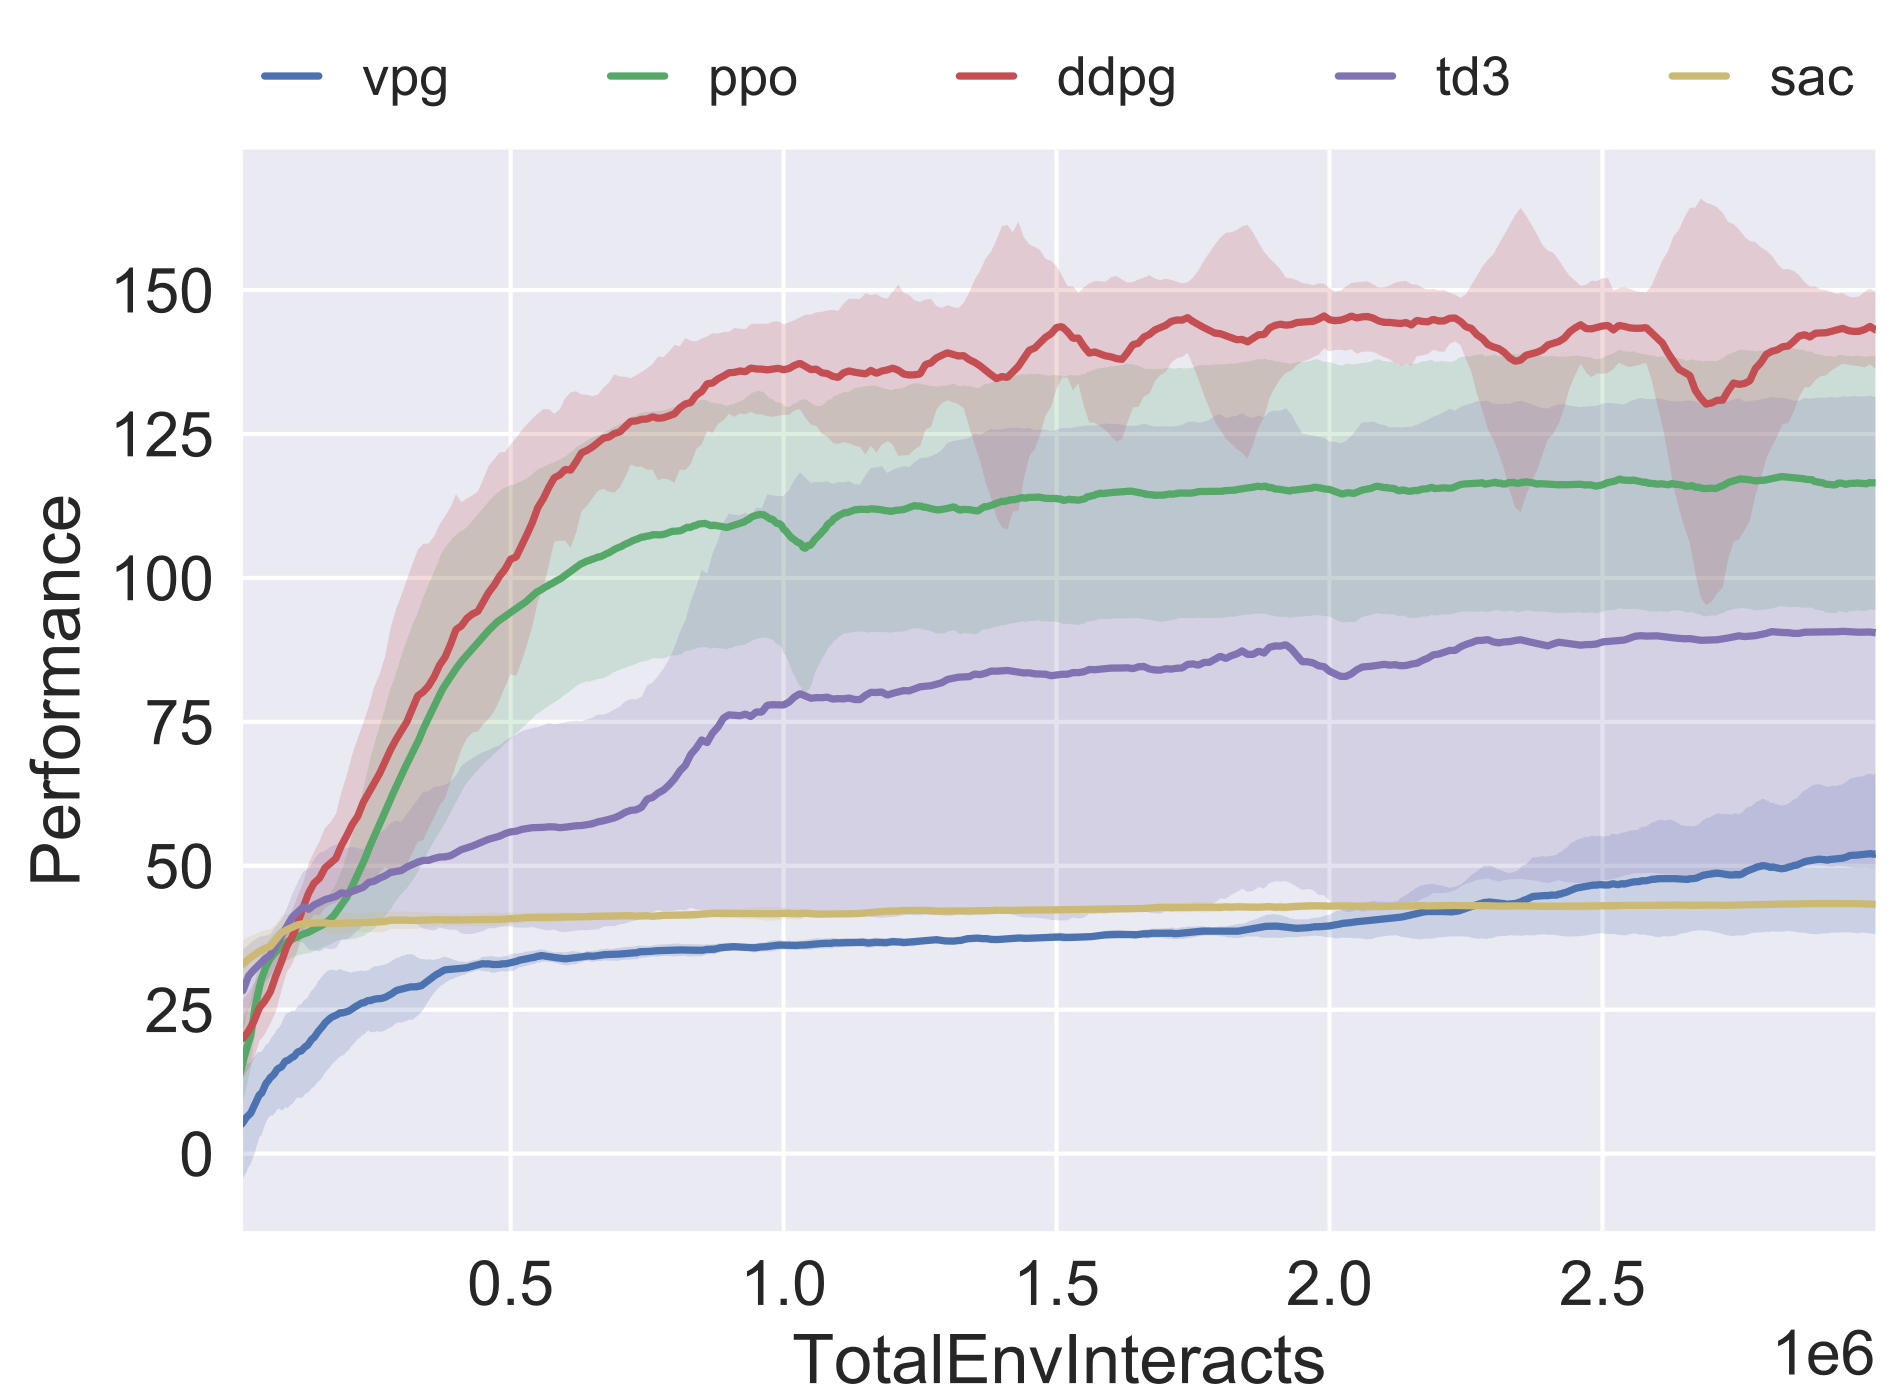
\includegraphics[scale=.2]{pytorch_swimmer_performance.png}\\
    Figure \textbf{2}: Performance Comparison in Swimmer environment
\end{center}

\vspace{0.5cm}

\begin{center}
    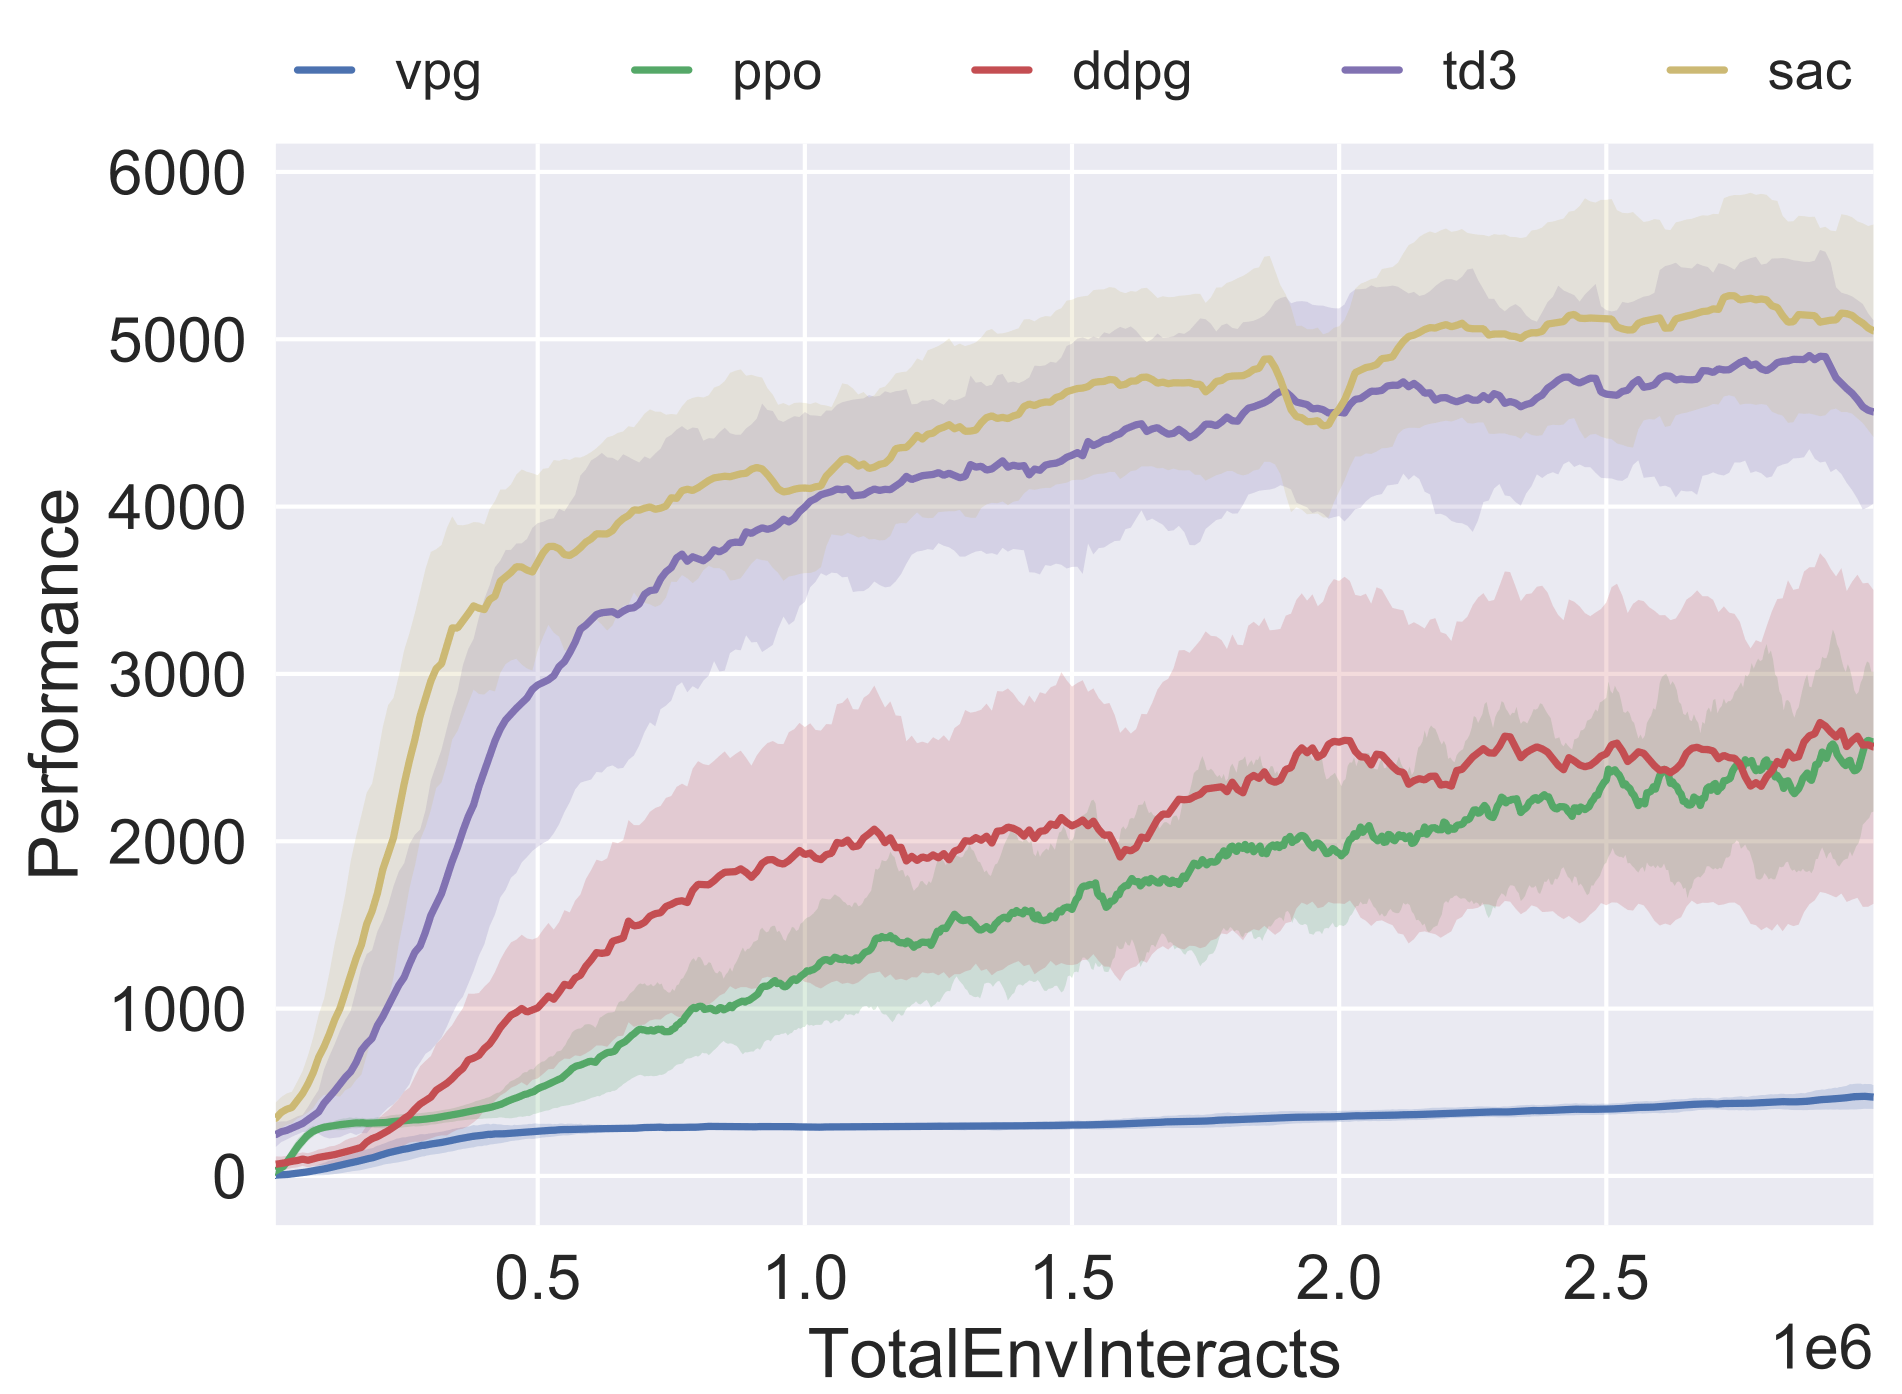
\includegraphics[scale=.2]{pytorch_walker2d_performance.png}\\
    Figure \textbf{3}: Performance Comparison in Walker2d environment \cite{spinup}
\end{center}
\vspace{0.5cm}
\noindent
We now apply the algorithm to the customised curling game play environment. One operation in the first implementation is to reset the current environment and reinitialise objects on the ice sheet. This original setting makes states independent to the each other, which may cause generalisation problems to the learnt policy. We test the performance of proposed approach with and without this step. The hyper-parameters and the architecture of networks remain the same in both groups, where only one group applies state reset. This comparison utilises the same evaluation metrics as in the algorithm competitors test. The values in table 2 suggest that learning on correlated states are beneficial to policy optimisation. The experience memory is capable of breaking the correlation while making use of the Markov property by mini-batch sampling. The original DDPG implementation is also compared as a baseline.
\newline
\newline
\noindent
The results of these experiments show that the applied TD3 algorithm for curling game play is of good stability and generalisation performance.
\vspace{1cm}
\begin{center}
    \begin{tabular}{|c|c|c|c|c|c|c|}
    \hline
    Iteration & 10k & 200k & 400k & 600k & 800k & \textbf{1m} \\
    \hline
    DDPG with reinitialised state & 1.57 & 2.33 & 2.51 & 2.57 & 2.84 & \textbf{2.97$\pm$0.39} \\
    \hline
    TD3 with reinitialised state & 2.15 & 3.12 & 4.31 & 4.44 & 5.01 & \textbf{5.18$\pm$0.41} \\
    \hline
    TD3 with sequential state & 2.05 & 4.47 & 5.41 & 5.89 & 6.22 & \textbf{6.32$\pm$0.23} \\
    \hline
    \end{tabular}
\end{center}
\begin{center}
    Table \textbf{2}: The test is run on 1 million time-steps with fixed batch size. \\ It shows  TD3 with sequential state returns a better and more stable policy.
\end{center}

\newpage
\section{Discussion}
We reflect on the conduction of this project in this section and discuss potential future developments to the current implementation.
\newline
\newline
\noindent
This project develops an direct approach to train the agent to play curling in the face of different settings. On the first look of this problem, the solution can be easily reached by simulating samples of plays. The key problem of such direct approach is that the featured representation of the current state is determined by the number of stones on the ice sheet. For instance, the coordinates of $m$ stones require at least $2m$ dimensions of observation. This limits the generalisation of the modelled task. The connected convolutional neural network improves the approximation capability of the model, which provides a better representation of visual input. The simulator of such task can record millions of frames of the process. The vanilla version of proposed method only makes use of the final image after the play. It can be argued that further development is possible to improve the sample efficiency of the algorithm. However, deep reinforcement learning algorithms are commonly accused of fitting too much data into a complex model.
\newline
\newline
\noindent
Comparing to a supervised learning method, we define the feedback of every sample with respect to the internal model of a curling game and learn to maximise the expected return of an action. In the first implementation, the stones on the ground are repositioned every episode, which breaks the dependence of samples to each other. Besides, the stochasticity in action space only affects the final rendering, skipping the collision frames. In every episode of the learning process, only one transition from the starting state to the finished state is considered. In the field of Markov decision process, this is a bandit problem that considers the next state reward as the expected return. We construct a variant of the task in the experiment where the positioning on the sheet remains after one play. The agent is faced with correlated states when learning to improve its policy. It is shown that the proposed algorithms still work but with less expected return. The experience replay mechanic is intended to break the correlation among experiences and enable stochastic gradient descent optimisation. However, the result shows a naive sampling method could be inadequate. Hindsight experience replay and prioritised replay methods weigh experiences  differently according to their target values. Further incorporation of a better off-policy experience sampling is potential to improve the algorithm in generalised adversarial settings.
\newline
\newline
\noindent
Our implementation of the RL algorithm is much more complex than the basic Markov process formulated in preliminaries. Generally, we combine three main ideas into the algorithm: function approximation, bootstrapping of estimate and off-policy training, also known as the *deadly triad*. It is argued that instability of model arises once all of them are present. Function approximator is essential to almost all reinforcement learning problems. A tabular representation alone is not a sufficient statistic for the inference of unseen states. Functions provide the power to scale to large problems and much greater expression with the help of deep neural networks. Bootstrapping method such as temporal-difference learning brings data efficiency to the process with the estimate over finite steps. It also enables the usage of incomplete episodes. For a large-scale problem, completing certain episode can cost huge in computation. Off-policy learning approach frees the behaviour from target policy so that the parameters can be updated individually. In a complex task, these are all necessary elements to formulate a model-free solution. Thus as shown in the development of methods, we mainly focus on the stabilisation of learning process caused by the deadly triad. This also makes it very hard to tweak the hyper parameters used in the implementations.
\newline
\newline
\noindent
An ideal formulation of curling game play should consider the competition between opposites. Self-play is one of the most classic method in reinforcement learning. It requires a competitive evolution strategy over agents through games against each other. One possible approach based on the current model is to swap the current team with opposite after each play. The aim of learning is also iterated over a maximised or minimised objective. A memory-based approach also suggests a better representation of states across different time steps. These proposed approaches suggest directions of future research.



\newpage
\section{Conclusion}
This project solves a task for the controllable agent to play curling in a simulated tabletop environment. We formulate the problem in a deep reinforcement learning model with variants in different settings. The agent progressively learns the control policy of the curling stone in the face of countless scenarios on the ice sheet. This project is aimed to explore the enormous research field of deep reinforcement learning for continuous control tasks. The proposed method applies twin delayed deep deterministic policy gradient method to a customised environment built in PyBullet simulator. The whole research process is established from the basis of reinforcement learning to state-of-the-art algorithms. Several modifications are conducted to suit the special case of this environment. The agent is able to learn end-to-end from the input rendered image for the purpose of maximisation of expected return. The internal model defined by the environment is in line with the rules of curling game, where rewards for the resulting states after collision are the difference in scores of both teams'. The results of experiments show that this approach is capable to generalise to variants of the formulated problems. This project is conducted with respect to a 12 weeks schedule. Although being interrupted by multiple accidents, it is considered to successfully complete the default objective. There is much room for improvement in the deep reinforcement learning researches. Future work is intended to explore the application of evolutionary strategy and meta learning in a RL setting.
\vspace{1cm}

\section{Appendix}
\subsection{Git repo}
The full developed software with algorithms and customised gym-curling environment is available at:
\\ \url{https://git-teaching.cs.bham.ac.uk/mod-msc-proj-2019/zxx992}
\vspace{1cm}
\subsection{Code structure}
The code structure of whole project is illustrated in the following figure:
\begin{center}
    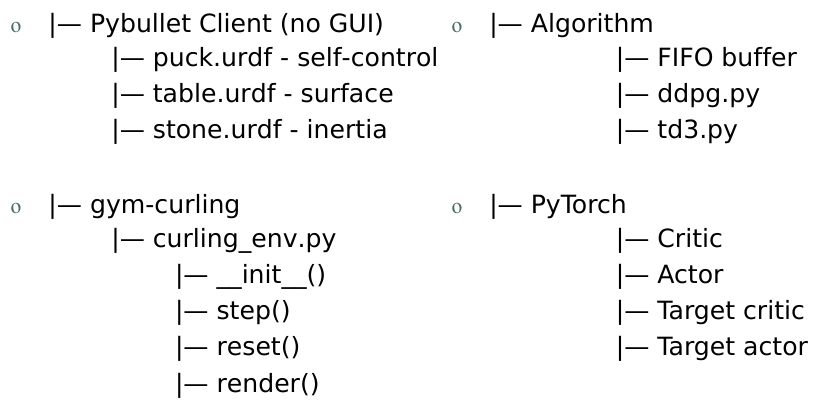
\includegraphics[scale=.4]{Arch.png}\\
    Figure \textbf{4}: Software architecture
\end{center}

\vspace{1cm}
\subsection{Testing}
To test the performance of algorithms, we need supplementary modules including \textit{Gym}, \textit{PyBullet}, \textit{mujoco}. We simply initiate the customised gym environment with suggested syntax and start testing inside the environment.



% Bibliography
\clearpage
\lhead{}\chead{MSc. Project Report \nouppercase{\leftmark}}\rhead{}
\phantomsection
\addcontentsline{toc}{section}{References}
\nocite{*}
\bibliography{mybib.bib}
\bibliographystyle{agsm}
\clearpage


\end{document}



